\documentclass[12pt,letterpaper]{article}

% ---------- Packages ----------
\usepackage[letterpaper,margin=1in]{geometry}
\usepackage[T1]{fontenc}
\usepackage[utf8]{inputenc}
\usepackage{newtxtext,newtxmath} % Times-like font
\usepackage{microtype}
\usepackage{graphicx}
\usepackage{booktabs}
\usepackage{array}
\usepackage{tabularx}
\usepackage{enumitem}
\usepackage{titlesec}
\usepackage{xcolor}
\usepackage{hyperref}
\usepackage{fancyhdr}

% ---------- Colors (from Aspose export) ----------
\definecolor{brand}{rgb}{0.478431,0,0.235294}   % color_147093
\definecolor{accent}{rgb}{0.67451,0.078431,0.333333} % color_195788
\definecolor{textgray}{rgb}{0.2,0.2,0.2}        % color_80434
\definecolor{rulegray}{rgb}{0.866667,0.866667,0.866667} % color_249244

% ---------- Document styling ----------
\hypersetup{colorlinks=true,linkcolor=brand,urlcolor=accent,citecolor=brand}
\pagestyle{fancy}
\fancyhf{}
\lhead{}
\rhead{}
\lfoot{SE/CS 3RA3 — Fall}
\rfoot{\thepage}
\renewcommand{\headrulewidth}{0pt}
\renewcommand{\footrulewidth}{0.4pt}

\titleformat{\section}{\Large\bfseries\color{brand}}{\thesection}{0.75em}{}
\titleformat{\subsection}{\large\bfseries\color{brand}}{\thesubsection}{0.75em}{}
\titleformat{\subsubsection}{\normalsize\bfseries\color{brand}}{\thesubsubsection}{0.75em}{}

\setlist[itemize]{topsep=4pt,itemsep=2pt,parsep=0pt}
\setlist[enumerate]{topsep=4pt,itemsep=2pt,parsep=0pt}

% ---------- Title page ----------
\makeatletter
\def\@maketitle{%
  \begin{center}
    \vspace*{1.5cm}
    {\Huge\bfseries\color{brand} Our Awesome Project\par}
    \vspace{0.35cm}
    {\Large\itshape\color{accent} Requirements Standard Plan\par}
    \vspace{0.9cm}
    {\large Saad Salman, Author 2, Author 3\par}
    \vspace{0.25cm}
    {\normalsize Version 1, 2025-09-22\par}
    \vspace{1.5cm}
  \end{center}
}
\makeatother
\title{}
\author{}
\date{}

\begin{document}
\maketitle
\thispagestyle{empty}
\clearpage

\tableofcontents
\clearpage

% ---------- Academic Integrity Disclaimer ----------
\section*{Academic Integrity Disclaimer}
\addcontentsline{toc}{section}{Academic Integrity Disclaimer}
We would like to acknowledge that as dedicated students of McMaster University, we have thoroughly read and comprehended the Academic Integrity Policy published by the university. We are committed to upholding the principles of academic honesty and integrity in all aspects of our educational journey. We understand the importance of acknowledging the work and ideas of others, and we pledge to ensure that all our academic endeavors are conducted with the utmost originality and compliance with the university's policy.

We affirm that the content presented in this document is entirely our own, and any external sources used have been appropriately cited and referenced.

\medskip
\noindent\textbf{Saad Salman} \\
As I submit my work, I, Saad Salman, take full responsibility for the integrity of my work and promise to avoid any form of plagiarism, cheating, or dishonest behavior. This acknowledgment serves as a testament to my dedication to academic excellence and the fostering of a trustworthy academic community at McMaster University.

\medskip
\noindent\textbf{Author 2} \\
As I submit my work, I, Author 2, take full responsibility for the integrity of my work and promise to avoid any form of plagiarism, cheating, or dishonest behavior. This acknowledgment serves as a testament to my dedication to academic excellence and the fostering of a trustworthy academic community at McMaster University.

\medskip
\noindent\textbf{Author 3} \\
As I submit my work, I, Author 3, take full responsibility for the integrity of my work and promise to avoid any form of plagiarism, cheating, or dishonest behavior. This acknowledgment serves as a testament to my dedication to academic excellence and the fostering of a trustworthy academic community at McMaster University.

\medskip
\noindent\textit{Policy:} \url{https://secretariat.mcmaster.ca/app/uploads/Academic-Integrity-Policy-1-1.pdf}

\clearpage

% ---------- Control Information ----------
\section{Control Information}
\begin{table}[h!]\centering
\caption*{Versioning and Delivery}
\renewcommand{\arraystretch}{1.2}
\begin{tabularx}{\textwidth}{@{}l l l l l l@{}}
\toprule
\textbf{Version} & \textbf{Delivery Deadline} & \textbf{Delivered} & \textbf{Feedback Received} & \textbf{Integrated} & \textbf{Notes} \\
\midrule
V1 & & & & & \\
V2 & & & & & \\
V3 & & & & & \\
\bottomrule
\end{tabularx}
\end{table}

\medskip
\noindent\textbf{Saad Salman} \\
Here is a quick biography of Saad Salman. You can contact them at \href{mailto:salmam12@mcmaster.ca}{salmam12@mcmaster.ca}.

\medskip
\noindent\textbf{Author 2} \\
Here is a quick biography of Author 2. You can contact them at \href{mailto:a2@mcmaster.ca}{a2@mcmaster.ca}.

\medskip
\noindent\textbf{Author 3} \\
Here is a quick biography of Author 3. You can contact them at \href{mailto:a3@mcmaster.ca}{a3@mcmaster.ca}.

\clearpage

% ---------- (G) Goals ----------
\section{(G) Goals}
\subsection*{Reading Guide}
Goals are ``needs of the target organization, which the system will address. While the development team is the principal user of the other books, the Goals book addresses a wider audience: essentially, all stakeholders \cite{meyer2022}. It must contain enough information to provide---if read just by itself---a general sketch of the entire project. To this effect, chapter G.3 presents a short overview of the system and G.1 will typically include some key properties of the environment. As it addresses a wide readership, it should be clear and minimize the use of specialized technical terms. Together, G.1, G.2 and G.3 describe the rationale for the project. It is important to state these justifications explicitly. Typically, they are well understood at the start of the project, but management and priorities can change \cite{meyer2022}.

\subsection*{Control Information}
\begin{table}[h!]\centering
\caption*{Table 1. Our Awesome Project --- Versioning Information --- Goal Book}
\renewcommand{\arraystretch}{1.1}
\begin{tabularx}{\textwidth}{@{}l l l l l l@{}}
\toprule
\textbf{Section} & \textbf{Version} & \textbf{Lead} & \textbf{Delivered on} & \textbf{Reviewer} & \textbf{Approved on} \\
\midrule
G.1 & M1 & SS & Sept-21-2025 & SP & Sept-22-2025 \\
G.2 & M1 & SS & Sept-21-2025 & SP & Sept-22-2025 \\
G.3 & & & & & \\
G.4 & & & & & \\
G.5 & & & & & \\
G.6 & & & & & \\
G.7 & & & & & \\
\bottomrule
\end{tabularx}
\end{table}

\subsection{(G.1) Context and Overall Objectives}
Commuting to McMaster University presents significant financial and environmental challenges. Students, staff, and faculty spend between 150 and 250 dollars monthly on fuel, parking, or transit, which places an economic burden on them. At the same time, single-occupancy vehicles contribute to 36 percent of greenhouse gas emissions for Canadian universities, harming both local air quality and broader sustainability goals. Existing ridesharing solutions such as Facebook Marketplace, Kijiji, or Poparide do not provide sufficient verification or security, leaving users at risk of riding with unaffiliated strangers. The objective of Hitchly is to provide a safe, affordable, and reliable ridesharing platform tailored for the McMaster community. By verifying users through McMaster email accounts, Hitchly ensures trust, reduces costs, supports sustainability, and helps the university meet its long-term community and environmental goals. 

\subsection{(G.2) Current Situation}
Currently, McMaster commuters lack a centralized, trusted platform to connect drivers and riders within the university community. Those who rely on driving face steep monthly costs for gas and parking, while those taking transit encounter expensive or unreliable services. Informal ridesharing options exist, but they provide limited safety features and lack institutional alignment, making them unsuitable for building long-term trust. Students and staff often feel that available solutions are unsafe, inefficient, or financially burdensome. Hitchly seeks to fill this gap by providing a McMaster-specific application that facilitates secure ridesharing, reduces commuting costs, and lowers emissions. 

\subsection{(G.3) Expected Benefits}
New processes, or improvements to existing processes, made possible by the project's results. It presents the business benefits expected from successful execution of the project. This chapter is the core of the Goals book, describing what the organization expects from the system \cite{meyer2022}.
The pilot delivers clear, stakeholder-visible outcomes. Riders should see more affordable commutes (targeting approximately 20\% savings) while drivers receive meaningful cost offsets (around 40\%). We aim for reliable availability ($\geq$70\% ride-fill and $\geq$95\% on-time) so trips feel predictable from day one, with most new users completing a first ride within a week. The pilot targets a reduction in single-occupancy trips on campus and nearby (aiming for at least 10\%), easing parking pressure and congestion and reducing emissions. The service will be inclusive by default (targeting about 90\% match on stated accessibility preferences) and trusted through university-verified identities with a goal of very low incident rates. The university benefits from higher student satisfaction and sense of belonging, improved commuter equity, and better alignment with sustainability reporting---while maintaining privacy safeguards (goal: zero critical incidents). Broader community outcomes include cleaner air, calmer peak traffic, and greater participation in transit and shared mobility.

\begin{figure}[htbp]
  \centering
  % path is relative to the .tex file; create docs/SRS/images/ and put your file there
  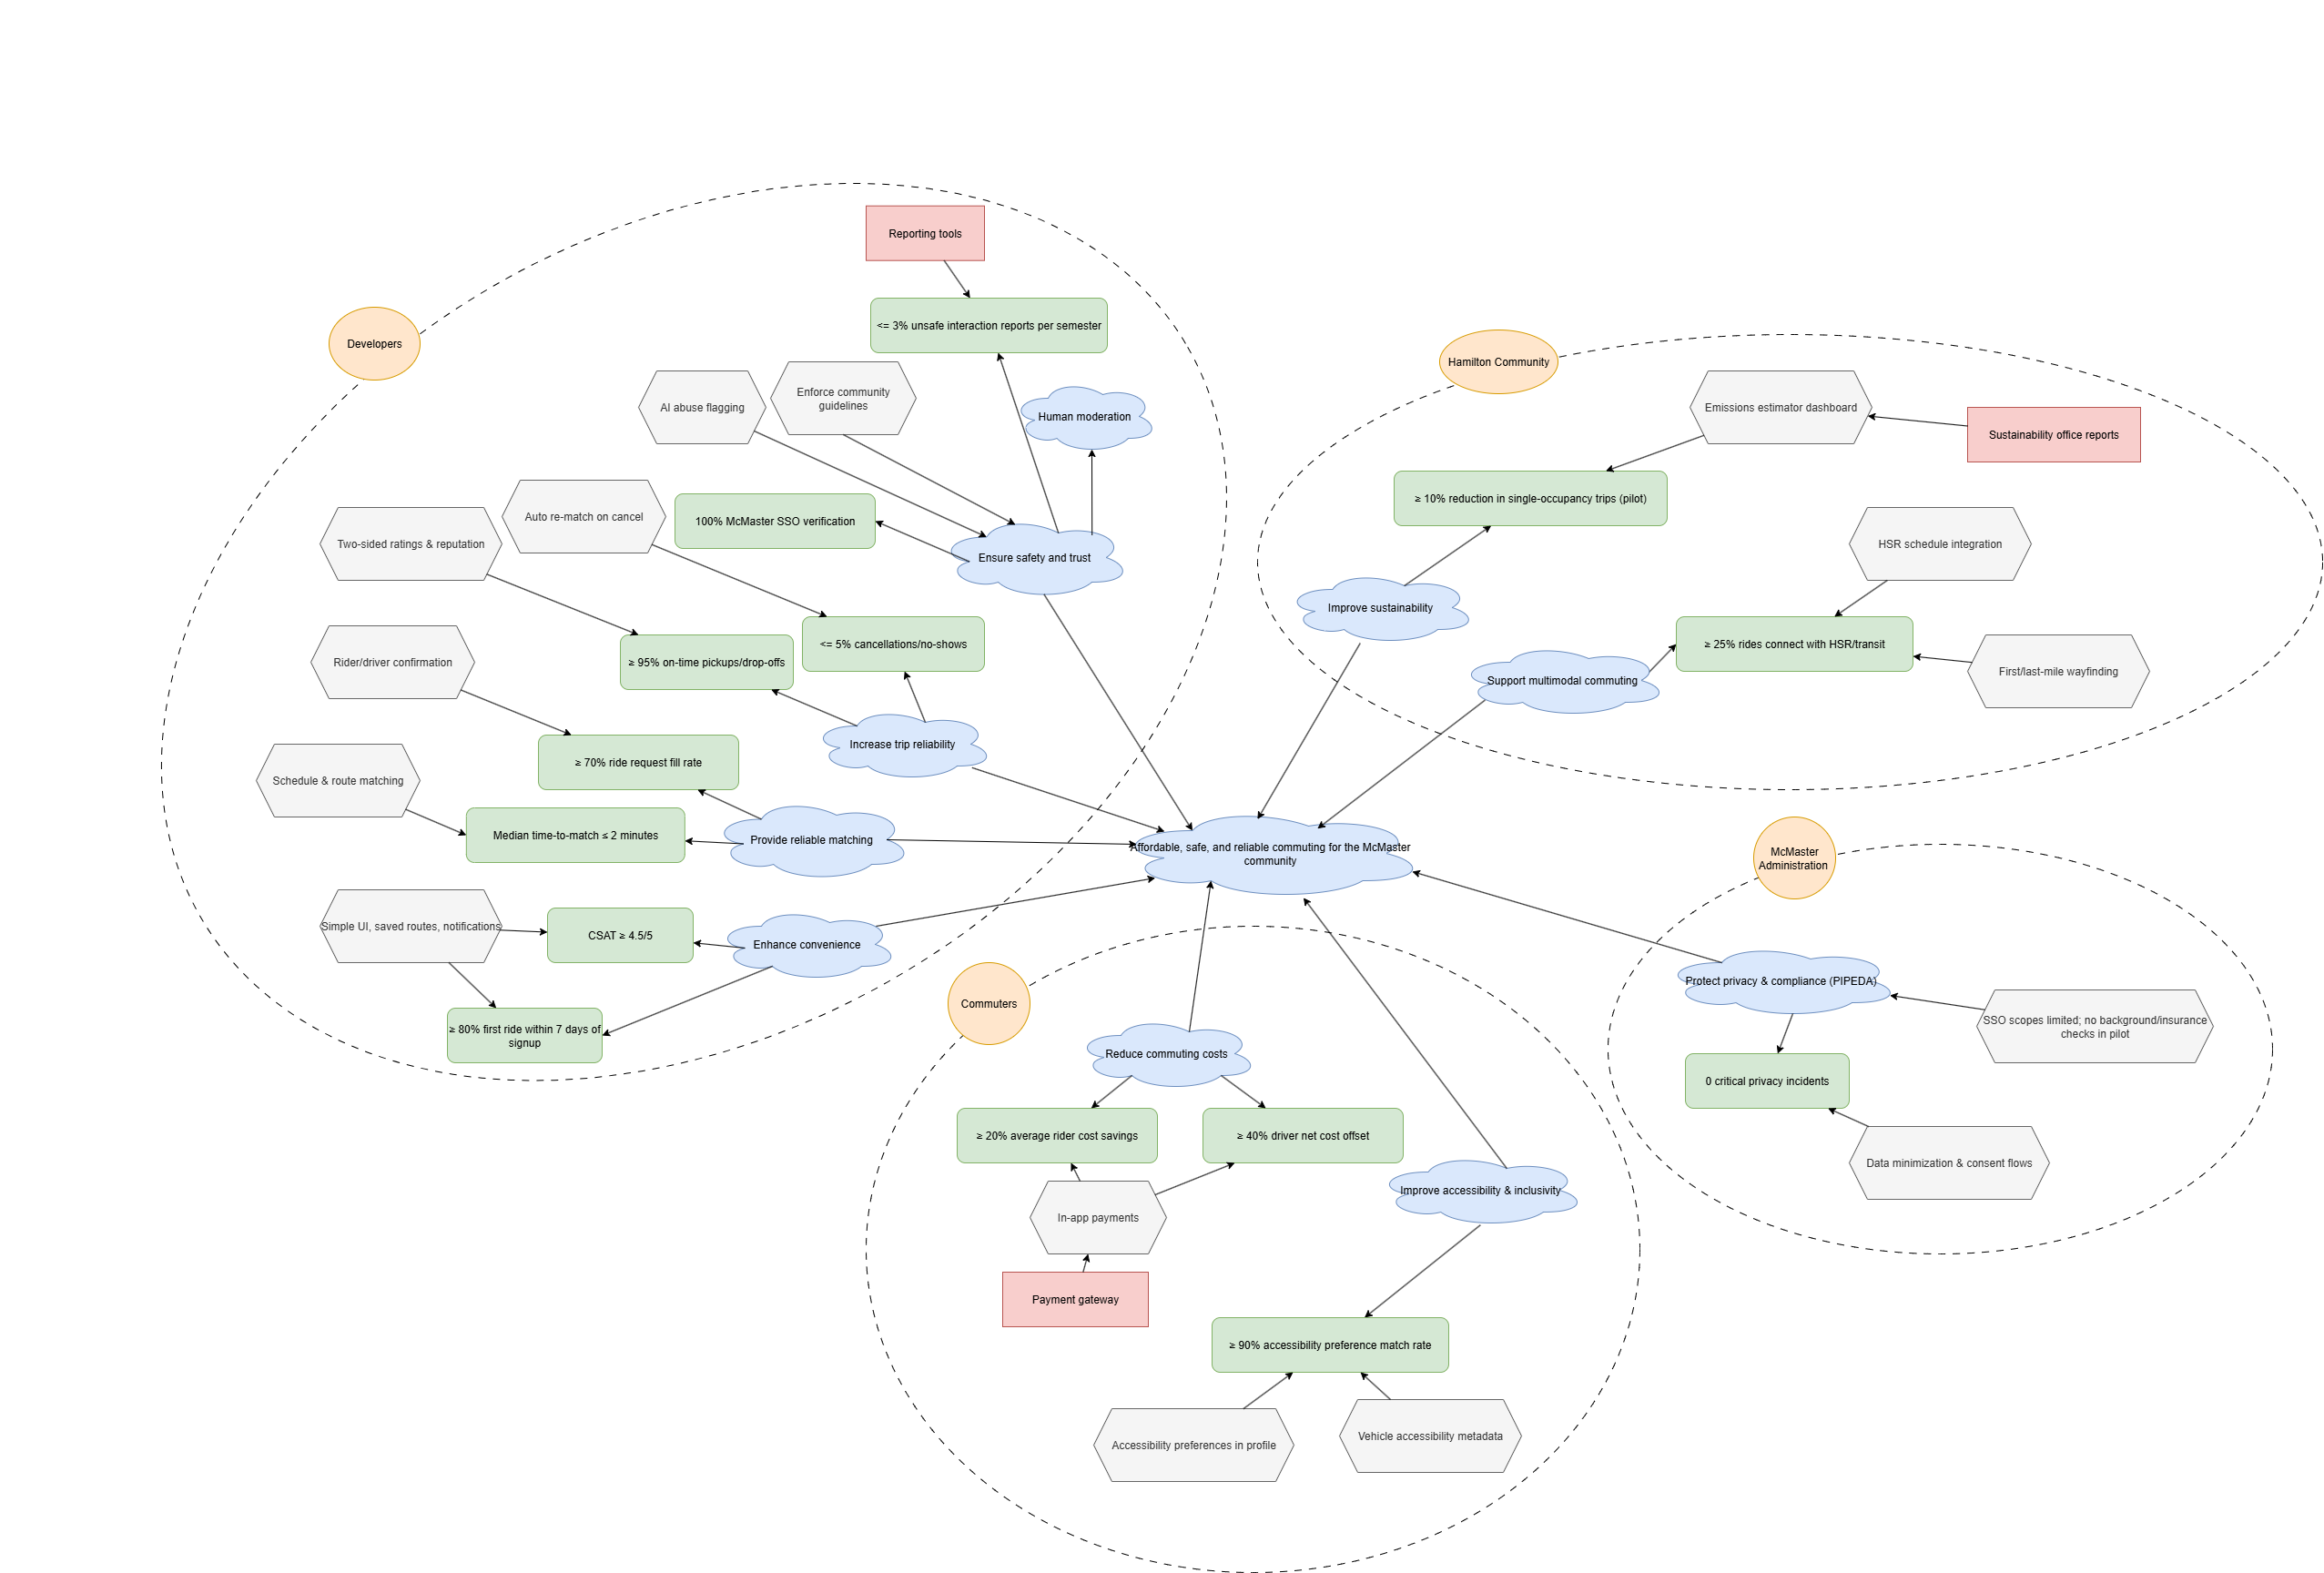
\includegraphics[width=0.75\textwidth]{goal_model.png}
  \caption{Hitchly Goal Modelling Diagram.}
  \label{fig:ride-matching}
\end{figure}

\textit{Nothing available at this point.}

\subsection{(G.4) Functionality Overview}

\paragraph{Overview.}
Hitchly is a campus-focused ride sharing service for the McMaster community.
It verifies users by McMaster email, collects commute and vehicle data, matches riders and drivers by schedule and location, estimates cost sharing, and supports post-trip ratings.

\subsection{(G.5) High-level Usage Scenarios}
Fundamental usage paths through the system, stated in user terms and independent of the system's structure. Detailed usage scenarios appear in the System book (S.4) \cite{meyer2022}.
\subsubsection*{Functional requirements}
\begin{enumerate}
  \item \textbf{User verification.}
  At sign-up, users must verify a McMaster-affiliated email address. Drivers additionally upload a valid driver's license for verification before being allowed to post rides.This two-level process ensures that all users are affiliated with McMaster and that drivers are properly credentialed.

  \item \textbf{Profile \& schedule input.}
  Riders and drivers provide basic profile details plus commute timetable, typical routes/areas, and preferences.
  Drivers additionally record vehicle and license information to enable appropriate matching and accountability.

  \item \textbf{Ride matching.}
  The system proposes compatible rider–driver pairings based on timetable overlap and approximate location.
  A match only becomes a trip after both sides confirm.

  \item \textbf{Cost estimate.}
  For each proposed trip, Hitchly computes a per-rider cost share that helps drivers offset expenses and helps riders save compared to solo travel.
  Estimates use driver-provided cost inputs at a simple, transparent level.

  \item \textbf{Ratings \& reviews (extension).}
  After trips, users can leave ratings and short reviews to inform future choices and encourage good behavior.
  These signals improve decision-making over time while remaining out of scope for the initial PoC.
\end{enumerate}

\subsubsection*{Most important two}
\textbf{User verification} and \textbf{Ride matching} are most important.
Verification directly addresses safety/trust, a primary adoption risk; matching is the core value creation that reduces search time and enables cost sharing. Together they validate the product’s viability and de-risk the project early.

\subsubsection*{Non-functional requirements}
\begin{enumerate}
  \item \textbf{Reliability (matching correctness).}
  Under typical peak usage, the matching function should consistently produce correct, reproducible pairings for the same inputs.
  Incorrect or inconsistent matches are treated as defects and prioritized in testing.

  \item \textbf{Usability (low-friction flows).}
  Common tasks (sign-up/verification, offering a ride, requesting a ride, confirming a match) should be understandable without training and completable in a small number of obvious steps.
  Clear labels and uncluttered presentation minimize onboarding time for first-time users.
\end{enumerate}

\subsubsection*{RACI for requirements}
\begin{center}
\begin{tabularx}{\textwidth}{@{}l c c c >{\raggedright\arraybackslash}X@{}}
\hline
\textbf{Requirement} & \textbf{Dev Team} & \textbf{Drivers} & \textbf{Riders} & \textbf{McMaster Univ. / Hamilton Community} \\
\hline
User verification & \textbf{R/A} & C & C & I \\
Profile \& schedule input & \textbf{R/A} & C & C & I \\
Ride matching & \textbf{R/A} & C & C & I \\
Cost estimate & \textbf{R/A} & C & C & I \\
Ratings \& reviews (extension) & \textbf{R/A} & C & C & I \\
Reliability (NFR) & \textbf{R/A} & C & C & I \\
Usability (NFR) & \textbf{R/A} & C & C & I \\
\hline
\end{tabularx}
\end{center}

\noindent{\textbf{Legend:}} R = Responsible (executes the work); A = Accountable (final sign-off); C = Consulted (provides input); I = Informed (kept up to date).

\subsection{(G.5) High-level Usage Scenarios}

\subsubsection*{Use Case 1: Driver Offers Ride}
\begin{enumerate}
    \item A driver registers with their McMaster email and drivers license.
    \item They input their schedule and vehicle details.
    \item Hitchly suggests potential riders with overlapping times.
    \item The driver confirms the riders they want to take.
    \item The system calculates cost-sharing estimates.
    \item After the trip, the driver receives ratings and reviews.
\end{enumerate}

\subsubsection*{Use Case 2: Rider Finds Ride}
\begin{enumerate}
    \item A rider signs up with a McMaster email.
    \item They enter their daily commute times and location.
    \item Hitchly presents a list of verified drivers with compatible schedules.
    \item The rider selects a driver and confirms.
    \item The system provides trip details, including cost share.
    \item After the ride, the rider leaves a review.
\end{enumerate}

\subsubsection*{Use Case 3: Report Safety Issue}
\begin{enumerate}
    \item A rider feels unsafe during a trip.
    \item They submit a report through the in-app reporting tool.
    \item Hitchly forwards the report to moderators.
    \item The moderators review and investigate the case.
    \item The driver’s or rider’s account is flagged if necessary.
    \item The system tracks the resolution and stores it for accountability.
\end{enumerate}

\subsubsection*{Use Case 4: Sustainability Tracking}
\begin{enumerate}
    \item Hitchly logs each completed trip.
    \item The system calculates estimated emissions avoided.
    \item Data is aggregated in dashboards.
    \item McMaster administration reviews statistics to measure impact.
    \item The results inform sustainability planning.
    \item Reports can be shared with the broader community.
\end{enumerate}

\begin{figure}[htbp]
  \centering
  % path is relative to the .tex file; create docs/SRS/images/ and put your file there
  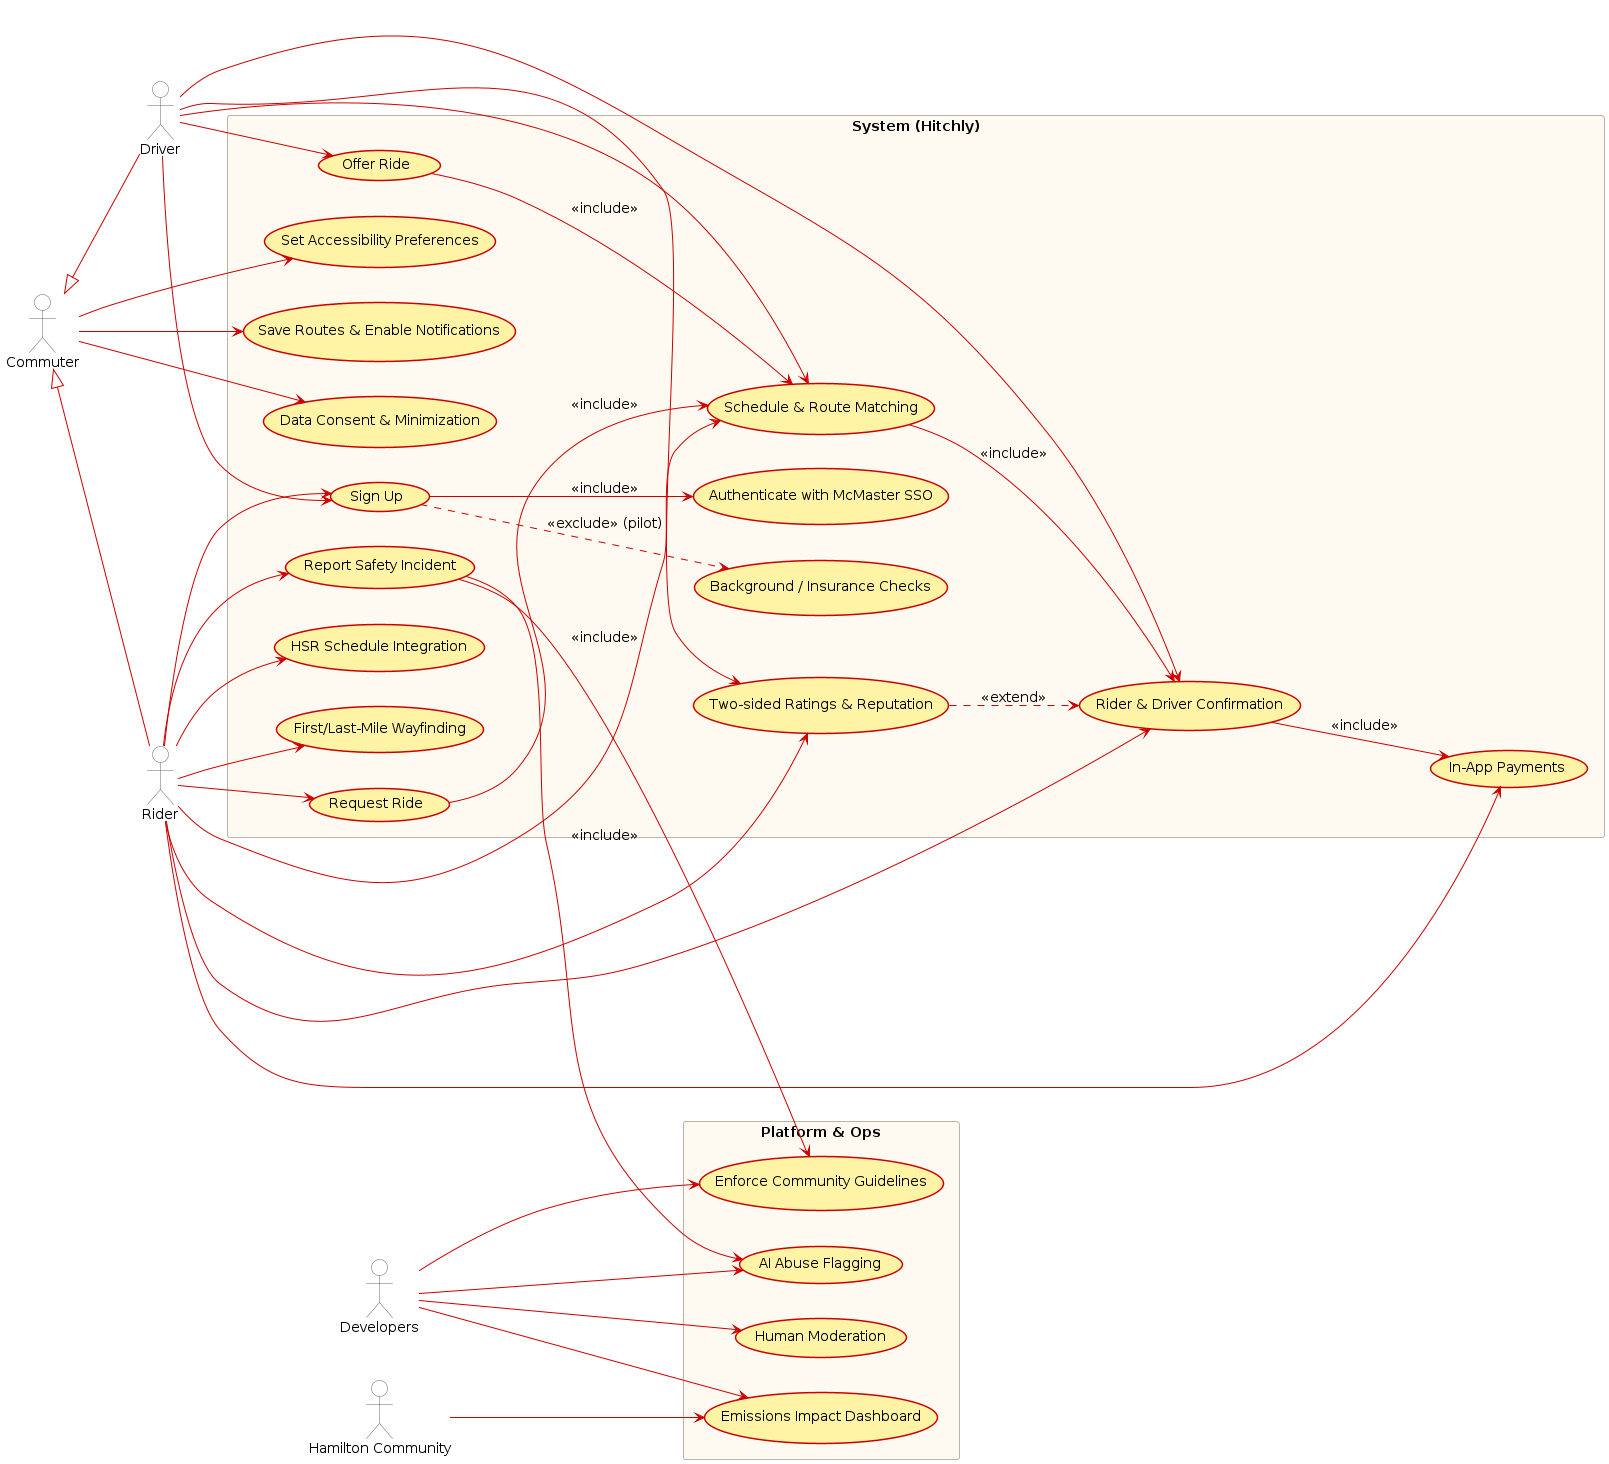
\includegraphics[width=0.75\textwidth]{use-case.png}
  \caption{Hitchly Use Case Diagram.}
  \label{fig:ride-matching}
\end{figure}

\subsection{(G.6) Limitations and Exclusions}
\begin{itemize}
  \item McMaster-Only Access: Hitchly will only be available to McMaster students, staff, and faculty during the pilot phase. Users must verify their identity through a McMaster email. This restriction ensures trust and control but limits the platform’s reach to a single institution. 

  \item Background and Insurance Checks: For the pilot phase, Hitchly will not perform in-depth background checks or validate driver insurance. Verification is limited to McMaster email zn d driver license authentication. This keeps onboarding simple but places responsibility on users to ensure their own compliance with driving regulations.

  \item Limited Route Flexibility: Hitchly will not provide dynamic routing or live GPS tracking during the pilot. Riders and drivers must coordinate based on general pickup and drop-off locations. This simplifies the system but may limit convenience compared to fully featured ridesharing platforms. 
\end{itemize}


\subsection{(G.7) Stakeholders and Requirements Sources}

\subsubsection*{Direct Stakeholders}

\paragraph{Students}
They are frequent commuters with tight budgets who will use Hitchly to save money and connect with peers. 
Relevant because they face high monthly commuting costs.\\
\textbf{Persona:} ``Sarah, a second-year student living off-campus, spends over \$200 monthly on commuting. She uses Hitchly to reduce expenses and meet fellow students traveling the same route.''

\paragraph{Staff}
Staff members travel daily to campus and benefit from both cost savings and reduced parking stress. 
Relevant because they often drive alone and bear significant expenses.\\
\textbf{Persona:} ``James, a staff member living in Burlington, drives to McMaster five days a week. Hitchly allows him to share costs and avoid the hassle of finding parking.''

\paragraph{Faculty}
Professors and teaching assistants need reliable commuting options. 
Relevant because faculty members often have predictable schedules that align well with ridesharing.\\
\textbf{Persona:} ``Dr.~Patel, a professor commuting from Toronto twice a week, finds Hitchly helpful to split costs and reduce environmental impact.''

\paragraph{Drivers}
Any McMaster-affiliated individual who owns a car and can offer rides. 
Relevant because they reduce their commuting costs by sharing expenses.Drivers must verify their identity by uploading a valid license before offering rides.\\
\textbf{Persona:} ``Ali, a graduate student with a car, uses Hitchly to cover his parking and gas by picking up two riders daily.''

\paragraph{Riders}
Any McMaster-affiliated individual who does not own a vehicle. 
Relevant because they rely on others to get to campus affordably.\\
\textbf{Persona:} ``Maria, an international student living in residence, relies on Hitchly to find rides for weekend trips to Hamilton downtown.''

\subsubsection*{Indirect Stakeholders}

\paragraph{McMaster University Administration}
Gains reduced congestion and measurable sustainability improvements, aligning with institutional goals.

\paragraph{Hamilton Community}
Benefits from fewer cars on the road, reduced emissions, and improved air quality.

\clearpage

% ---------- (E) Environment ----------
\section{(E) Environment}

\subsection{(E.1) Glossary}
\begin{itemize}
\item \textbf{Rideshare:} A service that allows riders to carpool with a single driver to reach a common destination.
\item \textbf{Drivers:} They are users that will provide rideshare services with their personal vehicles.  
\item \textbf{Riders:} They are users that will carpool to and from McMaster University.
\item \textbf{Working Condition:} A vehicle is in working condition if it has all necessary functions in the vehicle working. For instance, it must have functional head/tail lights, tires, engine, brakes, brake lights etc.
\end{itemize}
\\

\begin{figure}[h] 
    \centering
    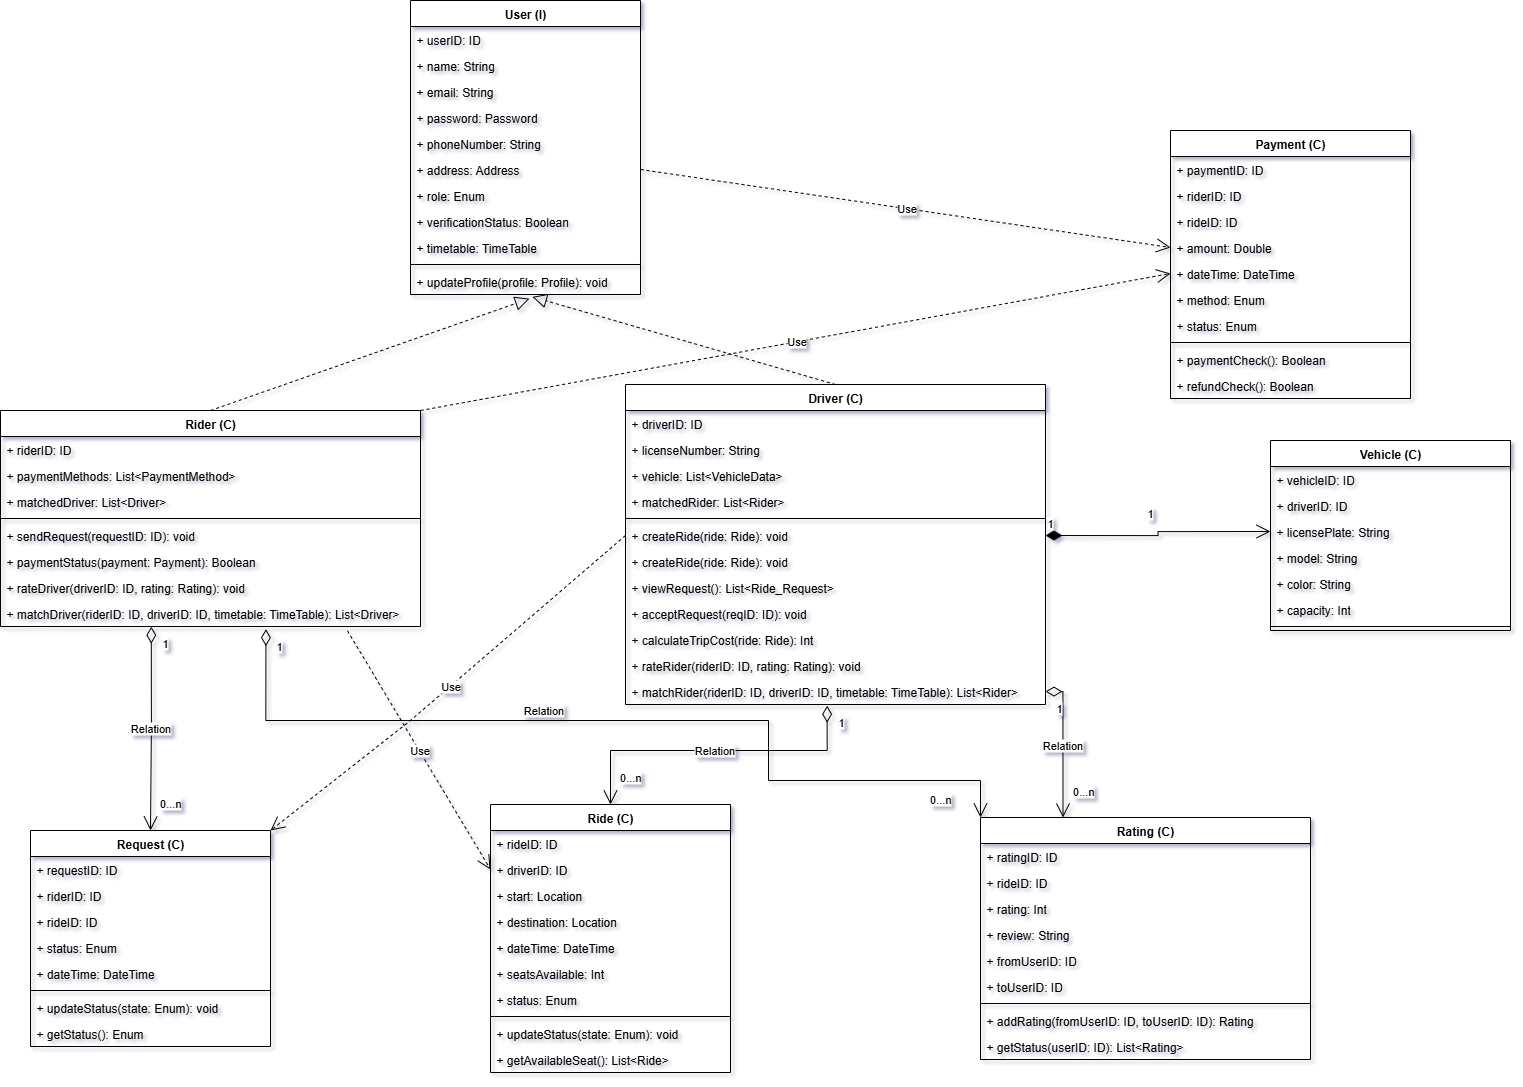
\includegraphics[width=0.8\linewidth]{Domain Model.png}
    \caption{Domain Model}
    \label{fig:domain-model}
\end{figure}

\subsection{(E.2) Components}
\begin{enumerate}
\item \textbf{MFA (Multi-Factored Authentication) Services:} The application will be interacting with components that will allow the application to verify users with their McMaster University emails with SMS/Phone verification. This is to ensure reliability and user trust.
\item \textbf{Payments Interface (i.e, Credit Cards, PayPal, Apple Pay etc.):} The application will also interact with a payment interface to allow for a smooth and streamlined payment process with Stripe. 
\item \textbf{Location API:} Google Maps will be used in several components of the application. This API will be used for location tracking, distance calculations, and for routing.
\end{enumerate}

\subsection{(E.3) Constraints}
These are a few limitations and restrictions coming from the environment onto the system: 
\begin{enumerate}
\item \textbf{Usage Constraint:} The project is currently limited and available to the McMaster community only. This would only include users that are currently students, staff members, or faculty members of the university. This application is currently limited to the Android and IOS operation systems. They will be compatible with any device with this operating system.
\item \textbf{Regulatory Constraint:} The project is constrained to comply with the PIPEDA laws and standards. This ensures that the user's data is handled carefully and with significant attention to maintaining data integrity and security. Each driver must have a Candian issued G2/G license, and the vehicle must be registered and insured. Each driver must comply with Ontario traffic rules and regulations. They must also not exceed the maximum passenger limit for their vehicle.
\item \textbf{Technical Constraints and Limitations:} A limitation of the Google Maps API is that it will be limited to providing minimal data for locations in rural areas. All functionalities in the applications must be completed in a limited time. For instance, the processing time for payments must be minimal. 
\end{enumerate}


\subsection{(E.4) Assumptions}
There are a few important assumptions that will be made to simplify the system. These will be assumed to be held, however, are not explicit constraints in the system.  
\begin{enumerate}
\item \textbf{User Behavior:} All users of the rideshare application will not intentionally cause any harm to each other during a trip. They will not misbehave or litter in the car. This is an important assumption as it ensures the safety of users and simplifies the process of carpooling.  
\item \textbf{Vehicle Condition:} Each driver has a vehicle that is in proper working condition. They are assumed to keep their vehicles clean. It will also be assumed that drivers will regularly maintain their vehicles.
\item \textbf{Language:} All users of the rideshare application must have a basic understanding of the English language, and they are able to communicate their thoughts with each other.
\item \textbf{User Base Demographic:} The application will assume a user base consisting of members of the McMaster University community. This may include students, staff, and faculty. This user group encompasses a diverse range of ages, genders, and ethnicities.
\item \textbf{Technical Compatibility and Reliability:} All third-party applications and API are assumed to be reliable. For instance, the Maps API will provide accurate data for all users in the GTA region. The API's rate limits will not exceed the expected user load. They are also assumed to have minimal downtime. 
\end{enumerate}

\subsection{(E.5) Effects}
Elements and properties of the environment that the system will affect \cite{meyer2022}. Effects of the application include:
\begin{enumerate}
\item \textbf{Improved sustainability and Reduced Traffic Congestion:} The system will positively affect the environment by lowering the GHG emissions caused by vehicles of individuals commuting to and from McMaster University. Secondly, as a result of carpooling, there will be a reduction in the use of single-occupancy vehicles which will cause a reduction in traffic congestion on roads and highways. 
\item \textbf{Usage of Public Transit:} There will be a significant reduction in the usage of buses and trains to commute to McMaster University because of the transition of people moving towards using the rideshare application, Hitchly. It may become convenient and affordable for commuters to use the rideshare services. Thus, resulting in a potential reduction in the usage of public transit.  
\item \textbf{UIncrease in Parking Spaces:} There can be an increase in available parking spaces due to the overall reduction of vehicles arriving at McMaster University. As a result of using the rideshare platform Hitchly, the number of single-occupancy vehicles will decrease. This would mean that fewer cars would arrive at McMaster University, reducing the overall demand for parking spaces.
\item \textbf{Increased Savings:} There can be an overall increase in the amount each commuter saves as a result of shifting to carpooling from other modes of transportation. Carpooling enables users to divide and share their cost, resulting in leaving them with more money in hand. 
\end{enumerate}

\subsection{(E.6) Invariants}
\begin{itemize}
\item Regular traffic will continue to move in Hamilton and surrounding areas where riders and drivers live. There can be traffic congestion on the roads due to car crashes and unusual weather conditions. There will also be times when an emergency vehicle may be on the roads occasionally, causing traffic congestion. These conditions will be present and will not change after the implementation of the application.  
\item The city of Hamilton will have and maintain their city infrastructure. There will be traffic lights, roads highways, pedestrian sidewalks, that will function normally.  The traffic rules and signs will be followed and maintained regardless of the implantation of the application. 
\item McMaster Parking systems will function as usual. There will not be any changes made to the parking rules or guidelines to specifically cater to the rideshare application users. 
\item Wi-Fi networks will operate independently and can become slow due to torrential weather conditions. Users may be affected by this as it can affect their accessibility to a Wi-Fi network during their ride. Lastly, the Wi-Fi networks function independently of the implementation of the application.  
\end{itemize}

\clearpage

% ---------- (S) System ----------
\section{(S) System}
The System book refines the Goals book by focusing on more detailed requirements.

\subsection{(S.1) Components}
Hitchly is composed of 6 main components that collectively provide the necessary functionality required for the application. \\

\noindent \textbf{Matchmaking Engine:} The matchmaking engine is responsible for matching riders with drivers based on schedules/timetables, departure times, routes and locations, and other user preferences. 
It interfaces with the scheduling system to ensure rides can be matched, whether it be one-time or recurring. It will optimize for cost, convenience, and schedule alignment. \\

\noindent \textbf{Scheduling and Booking Manager:} Allows users to upload their schedules to inform about their availability to facilitate matchmaking. It also ensures booked rides are stored, updated, or cancelled as per defined policies.  \\

\noindent \textbf{Safety and Verification Module:} This module provides secure login through McMaster email authentication. This ensures that only verified students and staff at McMaster may use the system, providing reassurance and safety for users and a sense of community. \\

\noindent \textbf{Payment and Cost Sharing System:} This system automatically calculates the cost of the ride for each rider based on the distance, number of passengers, gas, and parking costs. It manages in-app payment transactions and a transparent fee breakdown. \\

\noindent \textbf{User Profile Manager:} Stores user details such as a profile picture, bio, ratings, preferences, and more. Allows other users to view a profile when matching with each other to see information about them, as well as reliability metrics such as completed rides, any strikes, and more. \\

\noindent \textbf{Rating and Reputation System:} Tracks the attendance, punctuality, and safety related behaviour of drivers and riders. Issues strikes and penalties as needed, and integrates with the user profile manager to display user ratings and history. \\
\vspace{1em}

\begin{samepage}
\noindent The following diagram shows how these components interact and communicate when the application is being used.
\begin{figure}[!h]
  \centering
  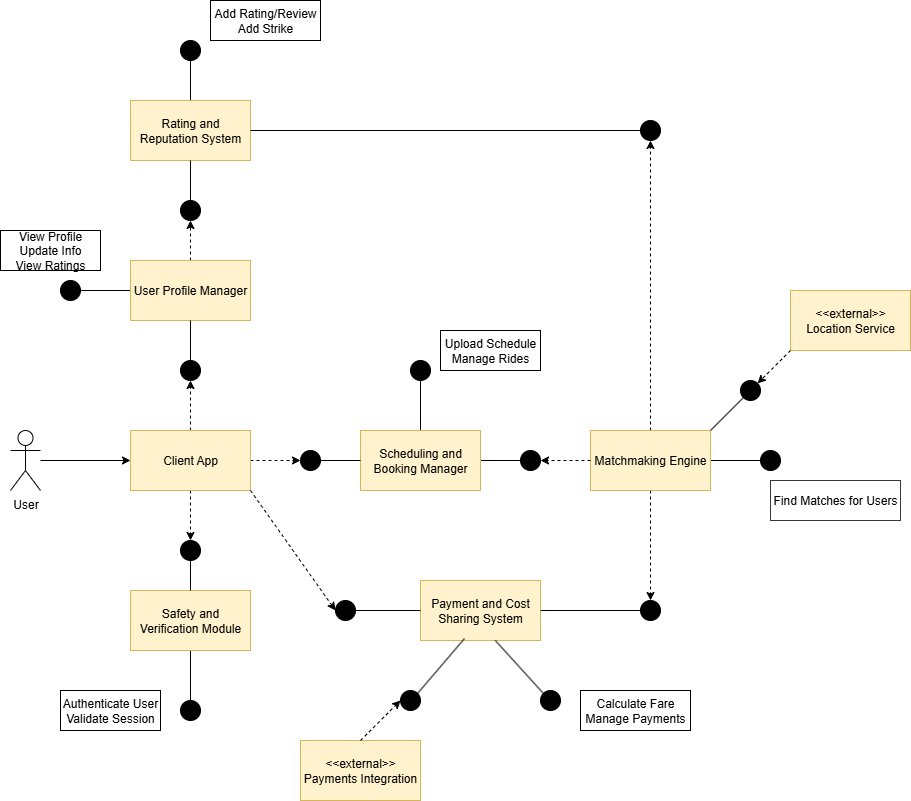
\includegraphics[width=0.9\textwidth]{component_diagram.png}
  \caption{Hitchly Component Diagram.}
\end{figure}
\end{samepage}
\clearpage

\subsection{(S.2) Functionality}
\textbf{Matchmaking engine} \\
\noindent Functional Requirements:
\begin{enumerate}
  \item Route and Schedule matching: The system shall compare driver routes and passenger locations to provide optimal ride matches.
  \item Availability Updates: The engine shall update available rides in real time as users create, edit, or cancel rides.
  \item Preference filtering: The engine shall allow users to filter matches by preferences, such as gender, music, vehicle type, etc.
  \item Multi-passenger support: The system shall allow for multiple passengers to match to the same driver, based on driver preference and vehicle capacity.
\end{enumerate}
Non-functional requirements:
\begin{enumerate}
  \item Matching performance: The engine shall generate ride matches within 10 seconds of a request.
  \item Location security: The engine shall ensure that user’s information used for matchmaking is not accessible outside of the development environment.
\end{enumerate}
\vspace{1em}
\noindent \textbf{Scheduling and Booking Manager} \\ 
Functional Requirements:
\begin{enumerate}
  \item Ride scheduling: Users shall be able to schedule rides in advance based on the results of the matchmaking engine.
  \item Booking confirmation: The system shall generate confirmations for bookings in the applications, and notify passenger(s) and the driver.
  \item Cancellation and Rescheduling: Users shall be able to cancel or reschedule rides within the specified timeframe and rules.
  \item Reminder notifications: The system shall send reminders to all passengers and the driver before any scheduled rides.
\end{enumerate} 
Non-functional requirements:
\begin{enumerate}
  \item Data Integrity: All booking data shall be securely stored and updated as required.
  \item Confirmation speed: Booking confirmations and changes shall be finalized and delivered to users within 5 seconds.
\end{enumerate}
\vspace{1em}
\noindent \textbf{Safety and Verification Module} \\
Functional Requirements:
\begin{enumerate}
  \item User Identity Verification: The system shall validate users through university email authentication in order to use the application.
  \item Driver Verification: The system shall store and verify driver license and vehicle registration information.
  \item Ride Check-in: The system shall prompt passengers and drivers to check in at the start and end of the ride.
  \item Safety check: The system shall keep track of any misconduct reported by users or any strikes on a user’s account.
\end{enumerate}
Non-functional Requirements:
\begin{enumerate}
  \item Data Security: Data used for verification shall be encrypted to ensure security.
  \item Auditability: The system shall maintain a log of all verification actions for at least 1 year.
\end{enumerate}
\vspace{1em}
\noindent \textbf{Payment and Cost Sharing System} \\
Functional Requirements:
\begin{enumerate}
  \item Fare Calculation: The system shall automatically calculate the costs for the ride for each passenger based on distance, number of passengers, parking costs, etc.
  \item Secure Transactions: The system shall support payment in the form of credit card, debit card, and other mobile wallet payment methods.
  \item Hold on Funds: The system shall put funds on hold until after a ride has been completed, in order to deal with cancellations or refunds.
  \item Expense Summaries: The system shall provide ride expense summaries and earnings reports for drivers.
\end{enumerate}
Non-functional Requirements:
\begin{enumerate}
  \item Transaction Security: Payments must be processed following security standards.
  \item Processing Speed: Transactions shall complete within 10 seconds of initiation.
\end{enumerate}
\vspace{1em}
\noindent \textbf{User Profile Manager} \\
Functional Requirements:
\begin{enumerate}
  \item Profile Creation: The system shall allow users to create profiles when signing up, including personal details and ride preferences.
  \item Profile Updates: The system shall allow users to update their profile information at any time.
  \item Ride History: The system shall store and display ride history and ratings for drivers and passengers.
  \item View Profiles: The system shall allow users to view profiles of other users when matched with them.
\end{enumerate}
Non-functional Requirements:
\begin{enumerate}
  \item Privacy: Any personal information used when signing up shall not be visible to other users.
  \item Performance: Profile data shall load within 2 seconds.
\end{enumerate}

\noindent \textbf{Rating and Reputation System} \\
Functional Requirements:
\begin{enumerate}
  \item Ride Ratings: The system shall allow users to rate each other after each ride.
  \item Issue Reporting: The system shall allow users to report any issues or misconduct that occurs during a ride.
  \item Minimum Reputation Thresholds: The system shall enforce a minimum rating for certain actions (e.g: Offering rides, hosting multiple passengers, joining scheduled rides, etc.).
  \item Positive Reinforcement: The system shall reward users who consistently obtain high ratings by giving out badges, titles, and more.
\end{enumerate}
Non-functional Requirements:
\begin{enumerate}
  \item Rating Integrity: The system shall detect and flag fradulent and spam reviews. 
\end{enumerate}


\subsection{(S.3) Interfaces} % S.3

Hitchly exposes its functionality through both user-facing interfaces and programmatic interfaces (APIs). These define how students, staff, and faculty interact with the application and how Hitchly integrates with external systems.

\subsubsection{(S.3.1) User Interfaces} % S.3.1

\paragraph{(S.3.1.1) Mobile App (Primary Interface)} % S.3.1.1
Hitchly is delivered as a cross-platform mobile app (iOS and Android via React Native/Expo). Users can:

\begin{itemize}
    \item Sign up and log in using McMaster email verification.
    \item Input personal data, commuting details, timetable, and location.
    \item Drivers can register their vehicles, upload license details, and set estimated trip costs.
    \item Riders can browse and request available rides that match their timetable and location.
    \item Both roles can view trip summaries, receive notifications, and use ratings/reviews.
    \item A clean, accessible UI built with NativeWind + shadcn/ui ensures usability.
\end{itemize}

\paragraph{(S.3.1.2) Notifications} % S.3.1.2
Push notifications (Expo notifications service) alert users when:

\begin{itemize}
    \item A match is found.
    \item A ride is confirmed or updated.
    \item A trip is completed with a generated summary.
\end{itemize}

\subsubsection{(S.3.2) Program Interfaces (APIs)} % S.3.2

\paragraph{(S.3.2.1) Hitchly Public API} % S.3.2.1
\begin{itemize}
    \item Authentication API: Validates McMaster-affiliated emails and issues JWT tokens.
    \item User API: Manages user accounts, profiles, schedules, and roles (driver/rider).
    \item Matching API: Exposes endpoints for submitting commute data, retrieving matches, and confirming trips.
    \item Trip API: Provides trip summaries, cost breakdowns, and trip history.
    \item Ratings API: Allows posting and retrieving ratings/reviews.
\end{itemize}

\paragraph{(S.3.2.2) Third-Party Integrations} % S.3.2.2
\begin{itemize}
    \item Email Verification: Integrates with McMaster’s email domain for signup restrictions.
    \item Mapping/Location Services: Uses a mapping provider (e.g., Mapbox or Google Maps API) to process geolocation and routing.
    \item Payment (future stretch): Possible integration with Stripe/PayPal for cost-sharing transactions.
\end{itemize}

Through these interfaces, Hitchly ensures safety (via controlled access), usability (via a student-focused app), and extensibility (via type-safe APIs).

\textit{Nothing available at this point.}

\subsection{(S.4) Detailed Usage Scenarios} % S.4

This section provides example interactions between users and Hitchly. Scenarios are written as user stories and include normal, special, and erroneous cases.

\subsubsection{(S.4.1) Rider Requests a Ride} % S.4.1
\begin{enumerate}
    \item Sarah, a second-year student, opens the Hitchly app and logs in with her McMaster email.
    \item She inputs her class timetable and home address.
    \item Hitchly suggests matching drivers commuting at similar times.
    \item Sarah requests a ride with a compatible driver.
    \item The driver accepts, and both receive a confirmation notification.
    \item After the ride, Hitchly records the trip and generates a summary.
\end{enumerate}

\subsubsection{(S.4.2) Driver Posts Availability} % S.4.2
\begin{enumerate}
    \item Omar, a graduate student, registers as a driver by submitting his license and car details.
    \item He enters his weekly commute schedule and estimated fuel/parking costs.
    \item Hitchly calculates a per-rider cost and displays suggested prices.
    \item Riders with compatible schedules can now request seats in Omar’s car.
    \item Omar accepts two riders and confirms the trip.
\end{enumerate}

\subsubsection{(S.4.3) Error Case — Invalid Email} % S.4.3
\begin{enumerate}
    \item A user attempts to register using a non-McMaster email.
    \item The system rejects the signup and prompts them to use a valid @mcmaster.ca email.
    \item The attempt is logged for auditing.
\end{enumerate}

\subsubsection{(S.4.4) Safety Case — Mismatched Data} % S.4.4
\begin{enumerate}
    \item A rider reports a driver whose profile information does not match their car/license.
    \item Hitchly flags the account and prevents further matches until the issue is resolved.
    \item Admins can review and verify the documentation.
\end{enumerate}

\subsubsection{(S.4.5) Ratings and Reviews} % S.4.5
\begin{enumerate}
    \item After a successful trip, riders are prompted to rate their driver on punctuality and safety.
    \item Omar receives a 5-star rating and positive feedback.
    \item His credibility score increases, making him more likely to be selected in the future.
\end{enumerate}

These scenarios highlight both standard use and exception handling, supporting the goals of affordability, safety, and sustainability.

\textit{Nothing available at this point.}

\subsection{(S.5) Prioritization}

\newcolumntype{Y}{>{\raggedright\arraybackslash}X}

\noindent \textbf{Priority Table for Matchmaking Engine}
\vspace{0.5em}
\begin{center}
\small
\begin{tabularx}{\textwidth}{|l|X|c|Y|}
\hline
\textbf{Requirement ID} & \textbf{Requirement Name} & \textbf{Priority Level} & \textbf{Reasoning} \\ \hline
F211 & Route and Schedule Matching & Must Have & Core feature of the app’s functionality. \\ \hline
F212 & Availability Updates & Must Have & Essential for reliability and real-time operation. \\ \hline
F213 & Preference Filtering & Should Have & Improves the user experience but not essential to core functionality. \\ \hline
F214 & Multi-passenger Support & Must Have & Having multiple passengers per driver is essential. \\ \hline
NF211 & Matching Performance & Should Have & Efficient algorithm and system is important for attracting users. \\ \hline
NF212 & Location Security & Must Have & It is essential that the user’s location information is kept secure. \\ \hline
\end{tabularx}
\end{center}
\vspace{2em}

\noindent \textbf{Priority Table for Scheduling and Booking Manager}
\vspace{0.5em}
  \begin{center}
  \small
  \begin{tabularx}{\textwidth}{|l|X|c|Y|}
  \hline
  \textbf{Requirement ID} & \textbf{Requirement Name} & \textbf{Priority Level} & \textbf{Reasoning} \\ \hline
  F221 & Ride Scheduling & Must Have & Core functionality of the app. \\ \hline
  F222 & Booking Confirmation & Must Have & Required for user trust. \\ \hline
  F223 & Cancellation and Rescheduling & Must Have & Essential for smooth operation for all users. \\ \hline
  F224 & Reminder Notifications & Nice to Have & Improves reliability but not critical for functionality. \\ \hline
  NF221 & Data Integrity & Must Have & Needed for user trust and safety. \\ \hline
  NF222 & Confirmation Speed & Should Have & Users will rely on quick confirmation to assess functionality. \\ \hline
  \end{tabularx}
\end{center}
  \vspace{2em}

  \noindent \textbf{Priority Table for Safety and Verification Module}
  \vspace{0.5em}
  \begin{center}
  \small
  \begin{tabularx}{\textwidth}{|l|X|c|Y|}
  \hline
  \textbf{Requirement ID} & \textbf{Requirement Name} & \textbf{Priority Level} & \textbf{Reasoning} \\ \hline
  F231 & User Identity Verification & Must Have & Required for the functionality and access of the app. \\ \hline
  F232 & Driver Verification & Must Have & Mandatory for trust and liability. \\ \hline
  F233 & Ride Check-in & Should Have & Ensures rides run smoothly but not essential. \\ \hline
  F234 & Safety Check & Nice to Have & Improves user safety and trust, but not critical for functionality. \\ \hline
  NF231 & Data Security & Must Have & Ensures that personal information is encrypted and securely stored. \\ \hline
  NF232 & Auditability & Nice to Have & Important for keeping track of user activity over time. \\ \hline
  \end{tabularx}
\end{center}
  \vspace{2em}
  
  \noindent \textbf{Priority Table for Payment and Cost Sharing System}
  \vspace{0.5em}
  \begin{center}  
  \small
  \begin{tabularx}{\textwidth}{|l|X|c|Y|}
  \hline
  \textbf{Requirement ID} & \textbf{Requirement Name} & \textbf{Priority Level} & \textbf{Reasoning} \\ \hline
  F241 & Fare Calculation & Must Have & Core functionality of cost-sharing. \\ \hline
  F242 & Secure Transactions & Must Have & Essential for user trust and legal compliance. \\ \hline
  F243 & Hold on Funds & Must Have & Needed for smooth functionality for all users. \\ \hline
  F244 & Expense Summaries & Nice to Have & Helpful for users to track budgets but not core functionality. \\ \hline
  NF241 & Transaction Security & Must Have & All payments must be handled securely for safety and legality. \\ \hline
  NF242 & Processing Speed & Should Have & Users will want a smooth process when completing payments. \\ \hline
  \end{tabularx}
\end{center}
  \vspace{2em}

  \noindent \textbf{Priority Table for User Profile Manager}
  \vspace{0.5em}
  \begin{center}
  \small
  \begin{tabularx}{\textwidth}{|l|X|c|Y|}
  \hline
  \textbf{Requirement ID} & \textbf{Requirement Name} & \textbf{Priority Level} & \textbf{Reasoning} \\ \hline
  F251 & Profile Creation & Must Have & Needed when signing up to use the application. \\ \hline
  F252 & Profile Updates & Must Have & Important for accuracy of information and preferences. \\ \hline
  F253 & Ride History & Should Have & Builds trust and data availability but does not directly improve functionality. \\ \hline
  F254 & View Profiles & Should Have & Important for user safety and trust when booking rides. \\ \hline
  NF251 & Privacy & Must Have & Protecting personal information is necessary for user confidence. \\ \hline
  NF252 & Performance & Nice to Have & Users will want fast navigation through information. \\ \hline
  \end{tabularx}
\end{center}
  \vspace{2em}

  \noindent \textbf{Priority Table for Rating and Reputation System}
  \vspace{0.5em}
  \begin{center}
  \small
  \begin{tabularx}{\textwidth}{|l|X|c|Y|}
  \hline
  \textbf{Requirement ID} & \textbf{Requirement Name} & \textbf{Priority Level} & \textbf{Reasoning} \\ \hline
  F261 & Ride Ratings & Must Have & Critical component of the rating system. \\ \hline
  F262 & Issue Reporting & Must Have & Important for evaluating and ensuring the safety of all users. \\ \hline
  F263 & Minimum Reputation Thresholds & Should Have & Enforces repurcussions for behaviour that goes against set rules, but not critical for functionality. \\ \hline
  F264 & Positive Reinforcement & Nice to Have & Provides benefits to users who consistently use the app as intended, but also not essential. \\ \hline
  NF261 & Rating Integrity & Should Have & Important to protect users reputations when possible. \\ \hline
  \end{tabularx}
\end{center}
\vspace{2em}

\par\raggedright
  The prioritization of requirements mainly focused on their importance to the app's core functionality, along with the safety and security of users and their data. 
  The core functionality refers to features that directly affect how users engage with Hitchly on a regular basis, such as finding and booking rides,
  managing payments, creating an account, etc. Requirements that are central to these experience are classified as "Must Have". Other features that provide
  significant improvements to convenience, trust, or improved user experience are categotized as "Should Have". Finally, features that offer additional ease of use
  or extra value but are not critical to the app's purpose are placed in the "Nice to Have" category.

\subsection{(S.6) Verification and Acceptance Criteria} % S.6

Verification and validation (V\&V) ensure Hitchly meets stakeholder expectations for usability, safety, and functionality. The following criteria define when the system will be considered satisfactory.

\subsubsection{(S.6.1) Module Testing} % S.6.1

\paragraph{(S.6.1.1) Authentication Module} % S.6.1.1
\begin{itemize}
    \item Accepts only @mcmaster.ca emails.
    \item Issues secure JWT tokens for valid accounts.
    \item Rejects invalid domains with appropriate error messages.
\end{itemize}

\paragraph{(S.6.1.2) Matching Engine} % S.6.1.2
\begin{itemize}
    \item Correctly pairs riders and drivers based on timetable and location inputs.
    \item Handles edge cases (no matches, multiple matches) gracefully.
\end{itemize}

\paragraph{(S.6.1.3) Trip Summary} % S.6.1.3
\begin{itemize}
    \item Generates accurate summaries with cost estimates.
    \item Stores records in PostgreSQL without data loss.
\end{itemize}

\subsubsection{(S.6.2) Integration Testing} % S.6.2
\begin{itemize}
    \item End-to-end tests ensure the mobile frontend communicates correctly with backend APIs.
    \item McMaster email verification integrates seamlessly with signup flow.
    \item Map/location services provide accurate routing data.
\end{itemize}

\subsubsection{(S.6.3) System Testing} % S.6.3
\begin{itemize}
    \item Hitchly runs on iOS and Android devices without critical crashes.
    \item UI components are accessible (WCAG AA compliance).
    \item Notification services deliver timely alerts for matches and trip updates.
\end{itemize}

\subsubsection{(S.6.4) User Acceptance Testing (UAT)} % S.6.4
\begin{itemize}
    \item Conducted with a group of McMaster students and staff.
    \item Success criteria:
    \begin{itemize}
        \item Users can sign up, request rides, and complete a trip without assistance.
        \item At least 80\% of participants report satisfaction with ease of use and reliability.
        \item No major safety concerns raised during trial.
    \end{itemize}
\end{itemize}

\subsubsection{(S.6.5) Static Analysis and Code Quality} % S.6.5
\begin{itemize}
    \item ESLint and Prettier pass on all commits.
    \item TypeScript compiler passes with no errors.
    \item Code coverage of unit tests $>$ 70\%.
\end{itemize}

\subsubsection{(S.6.6) Acceptance Criteria Summary} % S.6.6
Hitchly will be deemed acceptable if:

\begin{itemize}
    \item All core modules pass automated and manual tests.
    \item Integration tests confirm reliable operation across components.
    \item UAT demonstrates usability and trustworthiness.
    \item The system supports the project’s goals of affordability, safety, and sustainability.
\end{itemize}
\textit{Nothing available at this point.}

\clearpage

% ---------- (P) Project ----------
\section{(P) Project}

\subsection{(P.1) Roles and Personnel}
The team will consist of the following roles which have been pre-assigned based on qualifications:
\begin{itemize}
  \item \textbf{Project Manager (Swesan):}
  \begin{itemize}
      \item Oversee overall progress and deadlines
      \item Coordinate with TA and professor if needed
      \item Handle document submission
  \end{itemize}

  \item \textbf{Frontend Developer(s) (Burhan, Sarim):}
  \begin{itemize}
      \item Create mobile interfaces using design tools (Figma, Adobe XD)
      \item Develop user interface for the application using chosen development tools
      \item Integrate frontend UI with backend APIs
  \end{itemize}

  \item \textbf{Backend Developer(s) (Aidan, Hamzah, Sarim):}
  \begin{itemize}
      \item Develop server-side logic, APIs, and database connections
  \end{itemize}

  \item \textbf{Database Engineer (Burhan, Swesan):}
  \begin{itemize}
      \item Design database schema
      \item Optimize database queries
  \end{itemize}

  \item \textbf{Tester(s) (All team members):}
  \begin{itemize}
      \item Write and conduct test cases
      \item Document bugs and performance issues
      \item Collect user feedback
  \end{itemize}
\end{itemize}

\textit{\textbf{**All team members will be working on documentation**}}


\subsection{(P.2) Imposed Technical Choices}
The following imposed technical choices will apply:
\begin{itemize}
  \item \textbf{Programming Language \& Framework:}
  \begin{itemize}
      \item Must use languages/frameworks that all team members are familiar with.
      \item Mobile framework should be cross-platform to allow for both iOS and Android usage (React Native).
      \item Development machines will primarily run macOS and Windows; compatibility testing will be conducted for both.
  \end{itemize}

  \item \textbf{APIs / External Services:}
  \begin{itemize}
      \item Must use an external Maps API for routing and geolocation.
      \item Must use McMaster servers for hosting and storage (if permitted).
  \end{itemize}

  \item \textbf{Collaboration:}
  \begin{itemize}
    \item All code will be managed through GitLab repositories with protected main branches.
    \item Each feature will be developed in separate branches and merged via pull requests after peer review.
  \end{itemize}
\end{itemize}

\subsection{(P.3) Schedule and Milestones}

The project development will be divided into multiple sprints, each focusing on specific objectives and deliverables. This sprint-based approach ensures iterative progress and early testing of key functionalities.

\textbf{Sprint 1: Project Foundations (October)}
\begin{itemize}
    \item Finalize the technology stack for the application.
    \item Set up the development environment and ensure the mobile application environment runs on all developers’ hardware.
    \item Create Figma wireframes to map out the application flow.
    \item Design the initial database architecture for how information will be stored.
\end{itemize}

\textbf{Sprint 2: Create MVP (November)}
\begin{itemize}
    \item \textbf{Epic 1:} Implement fundamental features of the carpool application. \\
    \textit{As a user, I want to be able to connect with another user who has a similar schedule and a relevant commute route.}
    
    \item \textbf{Epic 2:} Implement basic payment features. \\
    \textit{As a user, I want to be able to complete a carpool session and split parking or fuel costs through the application.}
    
    \item \textbf{Minimal Viable Product (MVP):} \\
    The proposed Sprint 2 focuses on foundational features crucial for delivering a functional beta version of the application. The epics in this sprint implement Hitchly’s core functionality — carpool matching and basic payment — allowing for an initial user testing phase to validate the core system logic.
\end{itemize}

\textbf{Sprint 3: Core System Expansion (December)}
\begin{itemize}
    \item \textbf{Epic 3:} Add user verification. \\
    \textit{As a user, I want to ensure all application users are verified through their university email.}

    \item \textbf{Epic 4:} Add multi-passenger support. \\
    \textit{As a driver, I want to be able to connect to multiple passengers based on my vehicle capacity.}

    \item \textbf{Epic 5:} Add complex fare calculation. \\
    \textit{As a user, I want the system to calculate the fare for each passenger based on gas cost, number of passengers, and parking.}

    \item \textbf{Epic 6:} Add ride check-in. \\
    \textit{As a user, I want drivers and passengers to be prompted to check in at the start and end of each ride.}
\end{itemize}

\textbf{Sprint 4: Profile Addition (January)}
\begin{itemize}
    \item \textbf{Epic 7:} Add profile system. \\
    \textit{As a user, I want to create a personal profile to store my details and ride preferences.}

    \item \textbf{Epic 8:} Add profile updates. \\
    \textit{As a user, I want to be able to update my personal information at any time.}

    \item \textbf{Epic 9:} Add filtering to matching. \\
    \textit{As a user, I want to filter matches by preferences such as gender, music, or vehicle type.}

    \item \textbf{Epic 10:} Add rating system. \\
    \textit{As a user, I want to rate and review other users that I carpool with.}
\end{itemize}

\textbf{Sprint 5: Final Feature Additions (February)}
\begin{itemize}
    \item \textbf{Epic 11:} Add ride scheduling. \\
    \textit{As a user, I want to schedule my ride in advance.}

    \item \textbf{Epic 12:} Add booking confirmation. \\
    \textit{As a user, I want to receive a confirmation for my ride booking and notify other users part of the same ride.}

    \item \textbf{Epic 13:} Add reminder notifications. \\
    \textit{As a user, I want to receive reminder notifications for my scheduled ride as the time approaches.}

    \item \textbf{Epic 14:} Improve rating and review system. \\
    \textit{As a user, I want the review system to influence user trust scores and matching priority.}
\end{itemize}

\textbf{Sprint 6: Testing and Finalization (March – April)}
\begin{itemize}
    \item Conduct unit, integration, and system-wide testing across all modules to ensure stability and reliability.
    \item Optimize application performance and fix any remaining bugs identified during testing.
    \item Conduct user acceptance testing (UAT) with a pilot group and incorporate feedback.
    \item Prepare final presentation materials, poster, and demonstration for the April capstone showcase.
\end{itemize}

\subsection{(P.4) Required Technology Elements}
\begin{itemize}
  \item \textbf{Compliance with Payment API:}
  \begin{itemize}
      \item The application requires a secure payment gateway API that will be integrated with Hitchly to allow passengers to pay drivers for their carpool sessions. 
      \item This technology will enable the secure processing of payments, transactions, and the generation of billing information.
  \end{itemize}

  \item \textbf{Compliance with Maps API:}
  \begin{itemize}
      \item The application relies on navigation and location data to match users for carpooling based on their current location and routes to the university. 
      \item This will require full integration with a Maps API that allows precise user tracking, location comparison, and real-time route navigation across the campus area.
  \end{itemize}

  \item \textbf{Authentication API:}
  \begin{itemize}
      \item The application requires a secure authentication system that can reliably handle user login details. 
      \item This API will be integrated with Hitchly to manage user access, verification, and login sessions.
  \end{itemize}

  \item \textbf{Database Management System:}
  \begin{itemize}
      \item A reliable DBMS is essential for storing and managing user accounts, trip history, and audit logs for safety purposes. 
      \item This system will comply with the Hitchly application requirements and will be responsible for secure data storage and retrieval.
  \end{itemize}
\end{itemize}

\subsection{(P.5) Risk and Mitigation Analysis}
Some of the risks present during development are listed below:

\begin{itemize}
    \item \textbf{Low User Adoption:} The concept of carpooling with other students may not initially be popular, as many students may prefer driving alone or using public transportation. This could lead to low user adoption, especially during the testing phase when beta testers are needed to identify bugs and provide feedback. Since Hitchly relies on a large user base to strengthen its matchmaking algorithm, a limited number of users could reduce match quality. One mitigation strategy for this risk is to begin recruiting beta testers early and develop promotional material highlighting the benefits of carpooling. Starting outreach early would help increase awareness and build a stronger user base to test the application effectively.

    \item \textbf{Inaccurate Campus Data:} The application utilizes on-campus information such as parking costs and parking lot locations. Any changes to this information during the course of development could lead to inconsistencies or inaccurate data within the application. A mitigation strategy for this risk is to periodically check in with McMaster Parking Services to ensure that all campus-related data remains accurate and up to date.

    \item \textbf{Lack of User Trust with Data:} Some users may hesitate to trust a student-developed application with their personal and payment information. This lack of trust could negatively affect user adoption and engagement. A mitigation strategy for this risk is to integrate reliable third-party payment APIs, such as Stripe, to handle transactions securely. Additionally, maintaining transparency with users about which API services and security measures are implemented will help build trust and confidence in the system.
\end{itemize}

\subsection{(P.7) Requirements Process and Report}
The requirements process will involve interaction with direct stakeholders identified in Section G.7.  
For each stakeholder, the type of interview, its objective, and the most important question to be asked are listed below.

\begin{itemize}
    \item \textbf{Student (Sarah):}
    \begin{itemize}
        \item \textbf{Type of interview:} Closed. The objective is to understand the willingness of students to participate in carpooling.
        \item \textbf{Question:} \textit{“What factors would motivate you to use a student-based carpooling service instead of public transportation or driving alone?”}  
        We aim to identify which features would most effectively encourage user adoption.
    \end{itemize}

    \item \textbf{Staff (James):}
    \begin{itemize}
        \item \textbf{Type of interview:} Open. The objective is to understand how staff members currently commute to work.
        \item \textbf{Question:} \textit{“What is your current mode of transportation to campus?”}  
        This question will help determine how large the potential staff user base is and identify commuting challenges the app could address.
    \end{itemize}

    \item \textbf{Faculty (Dr. Patel):}
    \begin{itemize}
        \item \textbf{Type of interview:} Closed. The objective is to understand what benefits faculty members might expect from using a carpooling application, as financial incentives may not be their primary motivation.
        \item \textbf{Question:} \textit{“What benefits would you expect from using a university-based carpooling application compared to your current commute method?”}  
        This will help gauge which features are most valued by faculty members.
    \end{itemize}

    \item \textbf{Driver (Ali):}
    \begin{itemize}
        \item \textbf{Type of interview:} Open. The objective is to understand what would motivate drivers to participate as drivers rather than passengers.
        \item \textbf{Question:} \textit{“What incentives would encourage you to become a driver in a carpooling application?”}  
        This question will help determine which incentives—such as cost-sharing or community benefits—are most appealing to drivers.
    \end{itemize}

    \item \textbf{Rider (Maria):}
    \begin{itemize}
        \item \textbf{Type of interview:} Open. The objective is to understand any concerns passengers may have when using a carpooling application.
        \item \textbf{Question:} \textit{“What are some concerns you may have about using a carpooling application that matches you with other users?”}  
        This will help identify safety measures and system features that can address potential user concerns.
    \end{itemize}
\end{itemize}

\clearpage

% ---------- References ----------
\begin{thebibliography}{9}
\bibitem{meyer2022} Bertrand Meyer. \textit{Handbook of Requirements and Business Analysis}. Springer, 2022.
\bibitem{sommerville1997} Ian Sommerville and Peter Sawyer. \textit{Requirements Engineering: A Good Practice Guide}. Wiley, 1997.
\end{thebibliography}

\clearpage
\section{Reflection}
\begin{enumerate} 

\item What went well while writing this deliverable?  \\
Burhan: \\
The team had a clear idea of what we were trying to achieve with this document. The template is organized very well. It covers all of the concepts that need to be discussed for requirements. Moreover, the team was very active in brainstorming ideas for certain sections (i.e, function requirements, invariants, etc.). Lastly the instructions provided for most sections were very clear and detailed, which helped me understand and write the document easily.  
\\

Sarim: \\
Our team used the last document as a learning process to build off on what we did wrong. We made sure to hold frequent group sessions to ensure we were all on the same page. This was extremely important for a document like the SRS as there are many different sections that require team members to stay on the same page and work towards one specific goal.
\\

Hamzah: \\
I believe our team did a good job of dividing the work evenly so we are each doing sections that relate to each other. Also, we got started early on this deliverable so everyone had adequate time to complete their sections. The meyer template was easy to follow once it was set up, allowing our work to be very organized. 
\\

Swesan: \\
Since I am currently taking 3RA3 (Requirements), much of the content felt familiar and directly applicable. This helped me understand the structure of the deliverable and made writing easier, since I could connect course concepts with what we were expected to produce. It also gave me confidence that our sections were aligned with best practices. 
\\

\item What pain points did you experience during this deliverable, and how did you resolve them? \\
Burhan:\\ 

For some sections, the instructions were a little ambiguous. For example, the environment section, the instructions for assumptions and constraints were very similar, making it a bit unclear on how to differentiate between those two sections. Moreover, the SRS and the Hazard Analysis document both had a section for listing assumptions. This caused some confusion while writing the deliverable as I was unsure of which section to provide more detail. I was able to resolve this by asking detailed and specific questions about the ambiguity and confusion with the sections and instructions to the TA during our informal discussions. 
\\

Sarim: \\
Since there was not one speciic SRS document to pick from, there was alot of decision making involved in terms of which sections were important for the rubric, and which information needed to be on the Hazard Analysis document rather than the SRS or vice versa. It was extremely useful for us to utilize our TA meeting and ask questions regarding any ambiguity we faced, and to contiously review the rubric.
\\
 

Hamzah: \\
The initial set up of the document was confusing at first since there are several SRS template options to choose from, all of which have different formats and content. Additionally, there seemed to be many sections that were redundant and/or repetitive between sections and documents, which required clarification from the TA during our meeting. This includes questions such as what diagrams are required, how many requirements are needed, and more. 
\\
 Swesan: \\
One of the main challenges was making the diagrams and ensuring everyone's parts of the document were consistent in style and content. At first, this caused some confusion and extra editing, but I resolved it by refining the diagrams carefully and coordinating with the team to keep formatting and tone aligned across sections. 
 \\

  \item How many of your requirements were inspired by speaking to your   client(s) or their proxies (e.g. your peers, stakeholders, potential users)? \\
 

  The stakeholders for our project are McMaster students and faculty that commute to campus, so this would include our team members and many of our peers. By discussing our pain points and desires for this application
  with other students who are commuters, we were able to get a better understanding of what our application needs to include to meet their standards and expectations. This includes many of the features mentioned in section S.2,
  since this covers what is expected for each major component in the system. 
 

  \item Which of the courses you have taken, or are currently taking, will help 

  your team to be successful with your capstone project. \\

One of the most helpful courses for the capstone project so far has been SFWRENG 3RA3 (Software Requirements and Security Concerns), as the main project in this course was following the Meyer Tenplate to write a requirements document. 
This was extremely useful for this deliverable in particular, but also for all documentation deliverables in general since we got experience and learned key concepts which can be carried over. 
Other helpful courses include SFWRENG 2AA4, SFWREND 3BB4 (Software Design I and II) as they gave experience working in a group on a development project, and learning key software engineering principles which will be helpful
for the development of our application. 
 

  \item What knowledge and skills will the team collectively need to acquire to 

  successfully complete this capstone project?  Examples of possible knowledge 

  to acquire include domain specific knowledge from the domain of your 

  application, or software engineering knowledge, mechatronics knowledge or 

  computer science knowledge.  Skills may be related to technology, or writing, 

  or presentation, or team management, etc.  You should look to identify at 

  least one item for each team member. \\

 

Burhan: \\

I have minimal experience working on building a full stack application. There are a few things that I would need to acquire knowledge about. Our application will be based on a stack including React Native, TypeScript, and PostgreSQL. I have a lot of experience working with SQL; however, I haven’t worked with PostgreSQL before. This is an area in which I need to do some research and practice. Moreover, as this course involves a lot of documentation, I also need to acquire some knowledge within this area to strengthen my grammar and formal writing skills.  

 \\

 Sarim: \\
 Since my experience has mainly been in web development, I will need to focus my learing on mobile development. We chose React Native based on our skillset, since alot of us had experience with React.JS in web development so the skill would be somewhat familiar to us. This choice still requires me to learn a new skill but since both are comparitively similar, it makes for an easy transition.
\\

Hamzah: \\

One of the main skills I will need to learn is TypeScript, as we plan to use it to develop the application. I have experience with languages like JavaScript and other typed languages like Java, however I have not used TypeScript before, so this will be a new experience for me which I will need to take time to learn and get familiar with to be able to contribute better to the development of the application. 
\\
 
Swesan: \\
For me, the most important skills are collaboration, coding, and motivation. Since this is a team-based project, being able to work effectively with others and keep everyone on track will be essential. I also want to improve my technical coding contributions especially with type script while maintaining the drive to push the project forward. 
\\

  \item For each of the knowledge areas and skills identified in the previous 

  question, what are at least two approaches to acquiring the knowledge or 

  mastering the skill?  Of the identified approaches, which will each team 

  member pursue, and why did they make this choice? 

 \\

Burhan:  \\

For PostgreSQL, I will read the documentation provided by the official website and then proceed to watch YouTube tutorials on the basics of how the technology works. The next step would be to learn how to use it efficiently in a full stack environment. For this as well, I will watch YouTube tutorials. For my writing skills, I will go over some formal grammar documentations online. Moreover, I will also practice what I have learned with grammatical exercises found online.  
\\

Sarim: \\
To learn mobile development in React Native, my initial plan is to follow a youtube tutorial that goes through the fundamentals of framework. Once I learn the fundamentals, I will take some time to create simple mobile applications and utilize documentation to support my development. I believe that to apply any skill you need to be fully understand the fundamentals. By watching an initial tutorial, I would truly understand what I need. Being able to work on simple applications will help reinforce the fundamentals and learn through making mistakes.
\\
 

Hamzah: \\

In order to familiarize myself with TypeScript, I plan to read documentation and go through video tutorials to get a good understanding of the fundamentals and how it can be used. Additionally, once I have a grasp of the basics, I will attempt practice questions and/or small applications to apply my understanding and improve. Being able to follow along is useful, but actually applying the knowledge is the best way to learn. 
\\

Swesan: \\
For collaboration and motivation, two approaches are: (1) actively communicating with teammates and holding regular check-ins, and (2) staying accountable by being on top of my own tasks and deadlines. For coding, I will continue practicing through team coding sessions and peer reviews. I plan to pursue these approaches because working closely with my team and staying consistent with my responsibilities will naturally build both my technical and teamwork skills. 
\\

\end{enumerate}
\end{document}